\chapter{Analysis of Results} % Chapter title
%
\label{ch:analysis}

\begin{figure}[h]
	\centering
	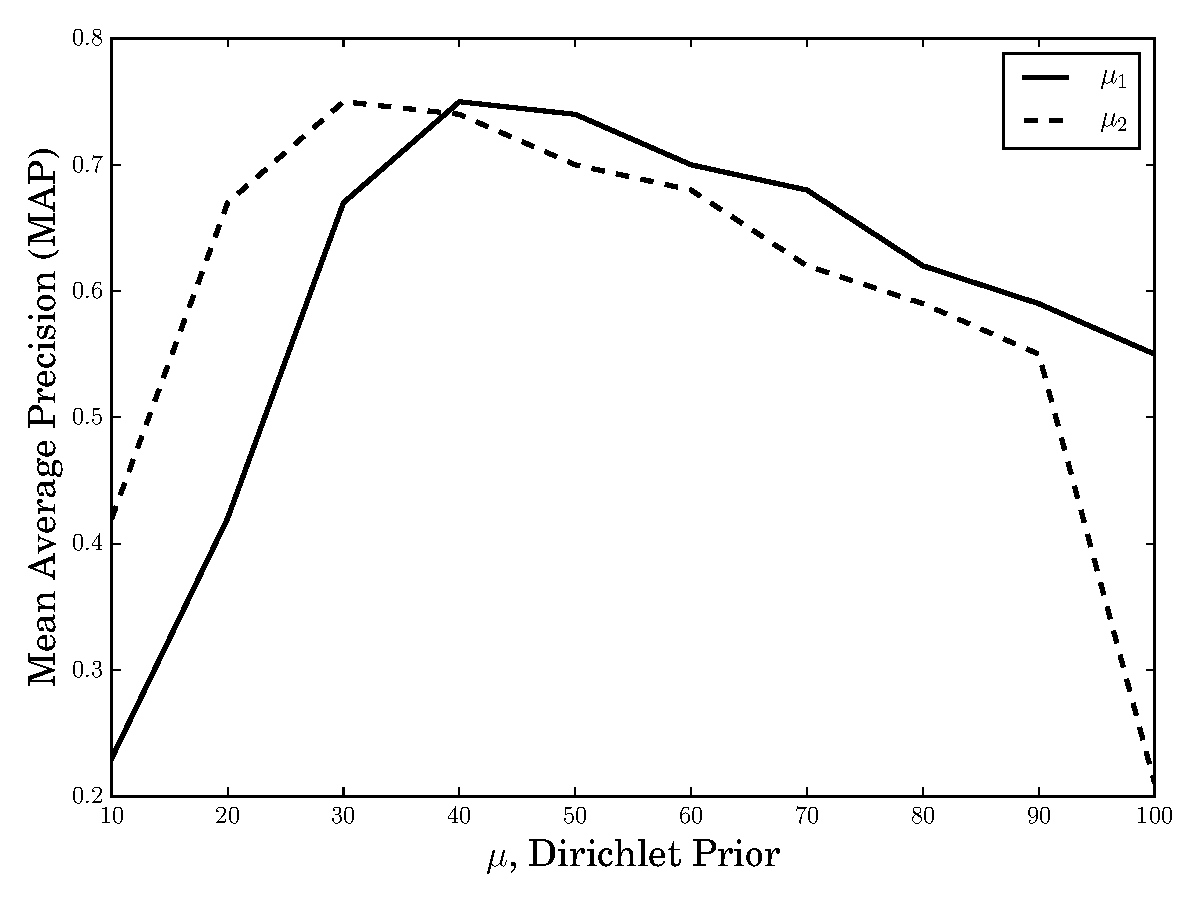
\includegraphics[width=\textwidth]{gfx/phew.pdf}
	\caption{Effect of Dirichlet prior against MAP with BREAK-2 ($\mu_1$) and with MAKE ($\mu_2$)}
	\label{phew}
\end{figure}

Before indexing the documents, the dataset must be split according to the desired BREAK variant.
For the usage of BREAK-n, note that one can store the positional vectors while indexing the corresponding term, or generate the vector directly during evaluation.
This choice highly depends on the time-space tradeoff.
However, in our experiments we have stored the vectors during indexing, prioritizing faster evaluation. 

\section{Analysis of Dirichlet Prior}

The common trend between the experimental setup is that Dirichlet tends to perform better than Okapi BM25.
This is due to the fact that Dirichlet prior smoothing factor, takes account the language modelling, which in turn, makes out to be more successful than vanilla BM25.
We investigate the effect of Dirichlet prior with BREAK-2 $\mu_1$ and with MAKE in $\mu_2$.
Figure \ref{phew} shows that both reach the maximum MAP equally, however $\mu_1$ reaches earlier.

\section{Analysis of Hyperparameters}

Now we analyze the effect of weighted average equation of MAKE, the hyperparameter tuning of the factor $\lambda$.
We investigate the effect of hyperparameter sensitivity in isolated spelling correction $\lambda_1$ and with cognate detection in $\lambda_2$.
\begin{figure}[h]
	\centering
	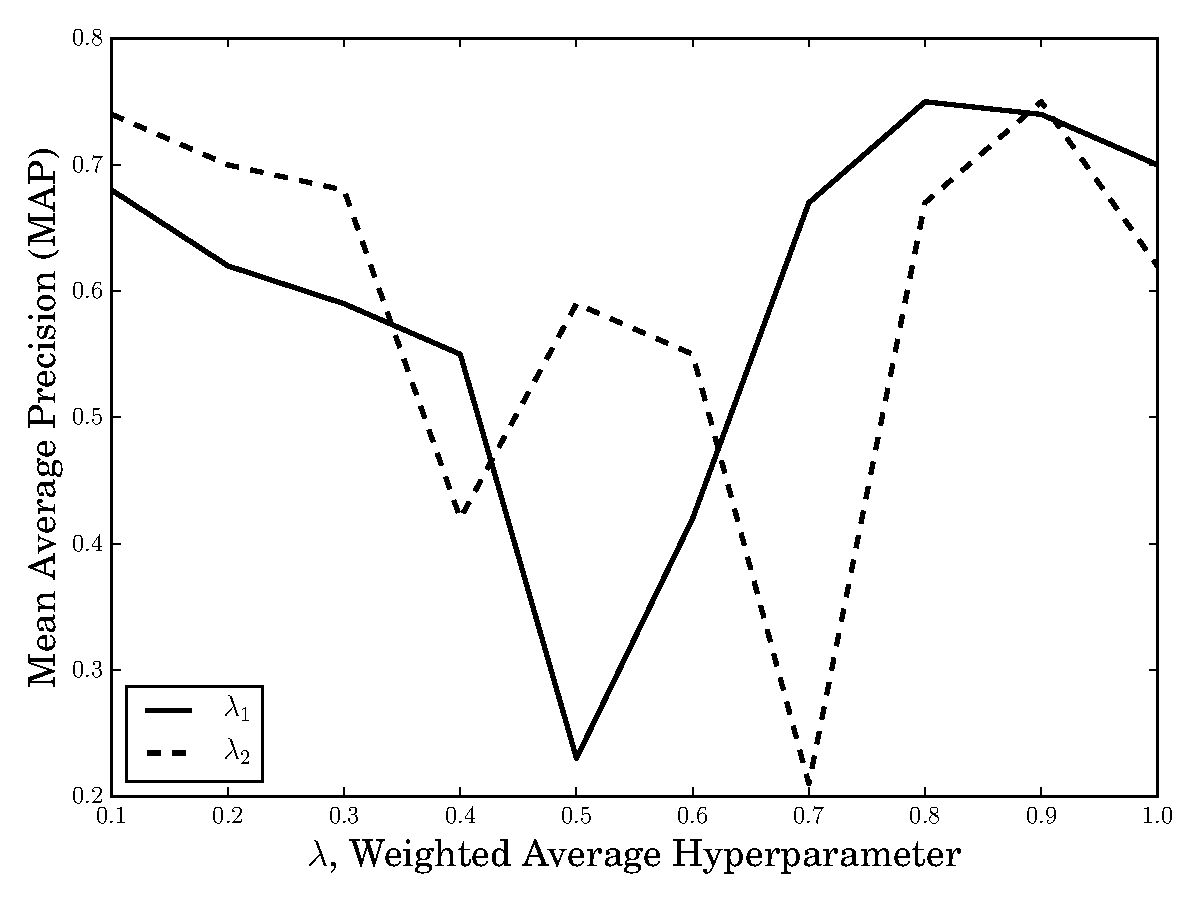
\includegraphics[width=\textwidth]{gfx/phew1.pdf}
	\caption{The effect of hyperparameter sensitivity in isolated spelling correction $\lambda_1$ and with cognate detection in $\lambda_2$.}
	\label{phew1}
\end{figure}

Figure \ref{phew1} describes the optimal conditions of the suitable hyperparameters.
The late reach of $\lambda_2$ suggests that cognate detection experiments depend more on graphical error modelling, MAKE algorithm than the BREAK heuristic.